\chapter{Design}

\section{Indledning}
Formålet med design afsnittet er at beskrive hardwaren og softwaren for EKG-systemet. Det beskrives med samtlige diagrammer og skitser for, at de forskellige klassers funktionalitet, og hvordan de snakker sammen klargøres.
  
\section{Hardware arkitektur}
I dette projekt er hardwaren blevet udleveret, så beskrivelsen af dette vil ikke  bliver beskrevet i yderste detalje. Hardwaren for systemet består af en National Instruments DAQ og en signalgenerator fra Analog Discovery. Disse er begge forbundet til en computer via USB-porte.
\\ 
I dette projekt bliver EKG-signalet ikke fysisk målt fra en patient, men simuleret fra et signal, som er hentet ned fra websiden PhysioNet \footnote{http://www.physionet.org}. 

\begin{figure}[H]
	\centering
	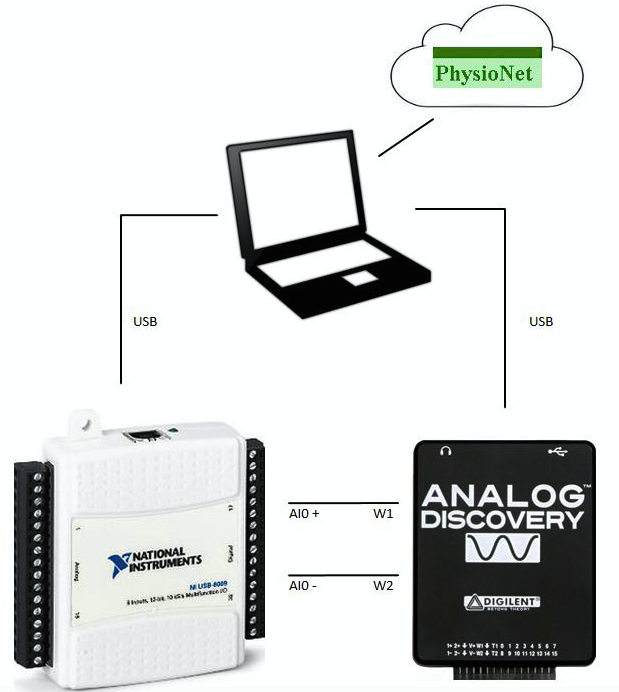
\includegraphics[width=0.6\textwidth]{Figurer/Snip20150427_1}
	\caption{Grafisk illustration af hardware opsætning}
\end{figure}

Som det ses på den overstående figur, er denne opstilling meget simpelt. Figur 2.1 viser, hvordan de forskellige komponenter relaterer til hinanden. Display hardwaren vil i dette projekt være en computer, da det kræver softwaren for at kunne vise EKG-signalet i form af en graf.
\\
\\  
Som beskrevet ovenfor er det Analog Discovery sammen med information for et EKG-signal fra PhysioNet, der skaber vores fiktive patient. Før EKG-signalet vises på computerens skærm skal det igennem de forskellige komponenter i opstillingen. Analog Discovery modtager EKG-signals  information som en CSV-fil, denne omdanner Analog Discovery til et analogt signal, som sendes videre til DAQ’en. DAQ’en digitaliserer det analoge signal, og tilpasser det, så det kan vises på computer skærmen. 

\subsection{Græseflader}
Grænseflader af forbindelserne imellem de forskellige dele af hardwaren. 

\begin{table}[H] 
	\begin{tabularx}{\textwidth}{l l X}
    \toprule
     \textbf{Forbindelse}   & \textbf{Signaltype} & \textbf{Funktionalitet}    \\ \midrule
     DAQ - Computer         & Digital & DAQ'en konverterer det analoge signal til digitalt og videresender det til 							  computeren. Informationen sendes begge veje. \\ 
     					      \addlinespace[2mm]                                                                                                                                                                            
     Computer - Analog Discovery			& Digital & Computeren simulerer et EKG-signal og sender det til Analog Discovery.\\ 
     				    	  \addlinespace[2mm]   				                                                                                                                                                                           
     Analog Discovery - DAQ			   	& Analog & Analog Discovery	 konverterer signalet fra digitalt til analogt og videresender det til 							      DAQ'en.\\  				      
    \bottomrule                                                                                                                   
    \end{tabularx}
    \caption {Beskrivelse af grænseflader.}
    \label{tab:graenseflader}
\end{table}



\section{Software arkitektur}
I dette projekt arbejdes der med objektorienteret programmering i programmeringssproget C\#. Dette er opbygget i henhold til trelagsmodellen, som er beskrevet i Rapporten under afsnittet Baggrund. Grafiklaget består af 4 GUI’er, logiklaget af en enkelt klasse, og datalaget består af 3 klasser, hvoraf den ene er en blackbox.

\subsection{GUI}
I dette afsnit vil GUI’erne nærmere beskrives. Grafiklaget består i alt af 4 GUI’er eller vinduer - Login-vindue, CPR-vindue, EKG-vindue og Gem\_måling-vindue.

\begin{figure}[H]
	\centering
	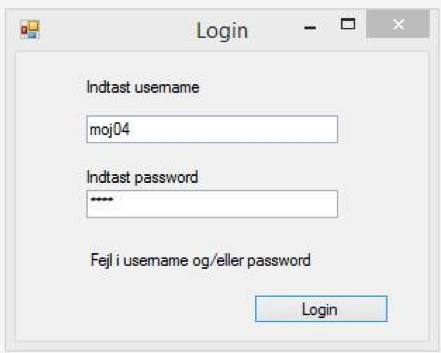
\includegraphics[width=0.8\textwidth]{Figurer/Snip20150430_38}
	\caption{Login-vindue}
\end{figure}

Når programmet startes op, vil et Login-vindue fremkomme på skærmen. Her skal brugeren logge ind for at få adgang til programmet. Hvis password og username ikke bliver godkendt, returnerer vinduet en fejl, i form af en linje tekst nedenunder indtast-felterne. Bliver login godkendt åbner CPR-vinduet.

\begin{figure}[H]
	\centering
	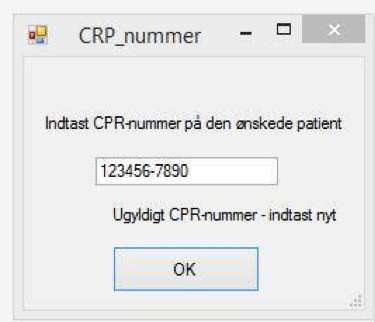
\includegraphics[width=0.6\textwidth]{Figurer/Snip20150430_39}
	\caption{CPR-vindue}
\end{figure} 

Her bliver brugeren bedt om at indskrive CPR-nummeret på den fiktive patient. CPR-nummeret bruges til at identificere personen i forbindelse med fremtidig måling samt gemme målingerne. Hvis CPR-nummeret ikke bliver godkendt, vil brugerne blive gjort opmærksom på dette via en fejlmelding. 
\\
\\
Når CPR-nummeret bliver godkendt, åbner det primære vindue, EKG-vinduet. 

\begin{figure}[H]
	\centering
	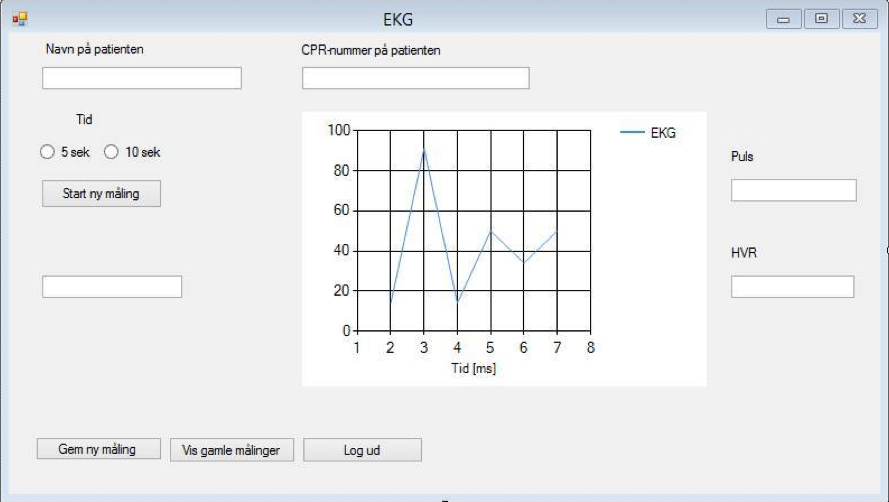
\includegraphics[width=1\textwidth]{Figurer/Snip20150430_40}
	\caption{EKG-vindue}
\end{figure}

EKG-vinduet er, hvor man kan køre og se målinger fra. Der er knapper til at vælge, hvor lang tid man ønsker en måling skal køre over. Til højre kan grafen for EKG-signalet ses, efter der er trykket ”Start ny måling”. Yderligere til højre kan der ses puls og HVR for den pågældende graf. Til venstre under knappen "Start ny måling" ses et tom tekstfelt. I dette tekstfelt vil diagnosen for EKG-signalet udskrives. Nederst er der knapper til at gemme målingerne, samt at logge ud fra programmet. Hvis man logger ud, kommer man tilbage til Login-vinduet. 
\\
\\
Det sidste vindue der er, forekommer når man trykker på ”Gem ny måling”. Her kommer der et pop-up vindue op, som bekræfter, at EKG-målingen er gemt. 

\begin{figure}[H]
	\centering
	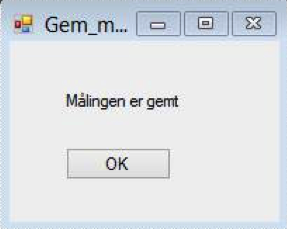
\includegraphics[width=0.5\textwidth]{Figurer/Snip20150430_41}
	\caption{Gem\_måling-vindue}
\end{figure}

\subsection{UML klassediagram}

\begin{figure}[H]
	\centering
	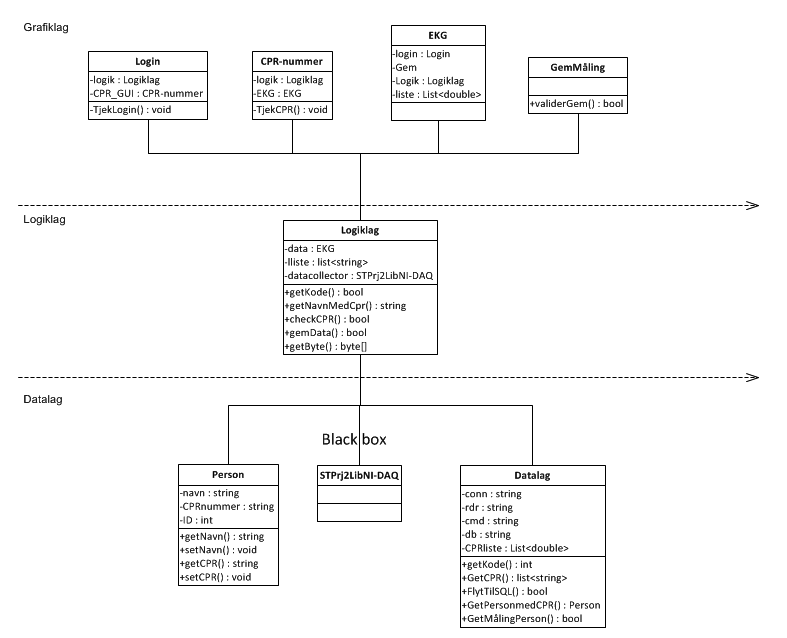
\includegraphics[width=1\textwidth]{Figurer/Snip20150430_42}
	\caption{UML-klassediagram over softwaren}
\end{figure}

\subsection{Appliktationsmodel}
Applikationsmodel vil i almindelig forstand indeholde en overordnet domænemodel, herefter klassediagram samt sekvensdiagram og tilsidst et opdateret klassediagram, hvor metoderne fra sekvensdiagram er inkluderet. 

Applikationsmodellen for dette projekt består af en overordnet domænemodel, herefter sekvensdiagram for de forskellige Use Cases med tilhørende opdateret klassediagram, som beskriver metodekald og kommunikation mellem klasserne. Klassediagrammerne er undladt, da de er irrevalt for dokumentationen for projektet. Applikationsmodellen er udarbejdet udfra Use Cases, hvilket medfører at metoderne er fiktive, altså ikke hentet direkte fra softwaren.  

\subsubsection{Domænemodel}
Domænemodellen er skabt på baggrund af de fem Use Cases. Gennem navneordanalyse af Use Casene er de konceptuelle klasser fundet. I modellen beskrives, hvordan de konceptuelle klasser interagerer med hinanden. Controlleren er ikke en konceptuelle klasse, men er den, der sørger for at systemet fungerer optimalt.
\\
Der er ingen multiplicity indsat i modellen, da der kun arbejdes med et scenarie af gangen. !!!!!!!!!!!!!!!!!!!!!!!!!!!!!!!! spørg Lars 

\begin{figure}[H]
	\centering
	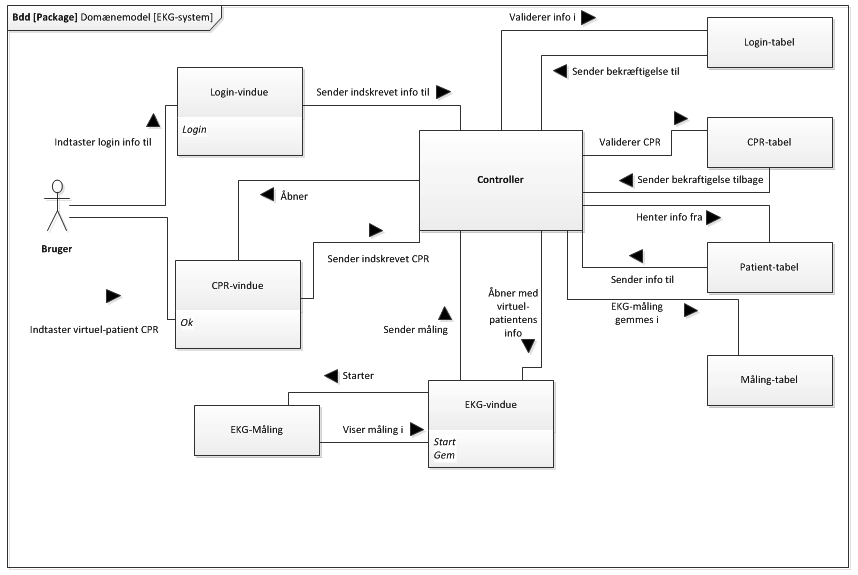
\includegraphics[width=1\textwidth]{Figurer/Snip20150429_37}
	\caption{Domænemodel af EKG-systemet}
\end{figure}

\subsubsection{Sekvensdiagram}
Sekvensdiagrammerne beskriver step-by-step via fiktive metoder forløbet i de forskellige Use Cases. Der er lavet et sekvensdiagram for hver Use Cases for at gøre systemet mere overskueligt. Et sekvensdiagram består af boundary-klasser og domain-klasser fra domænemodellen, samt en controller-klasse, som har navn efter den specifikke Use Case.  

\begin{figure}[H]
	\centering
	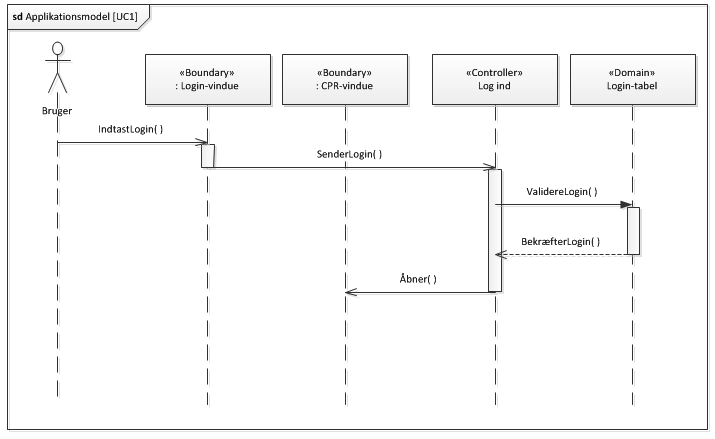
\includegraphics[width=0.9\textwidth]{Figurer/Snip20150429_34}
	\caption{Sekvensdiagram for UC1}
\end{figure}

\begin{figure}[H]
	\centering
	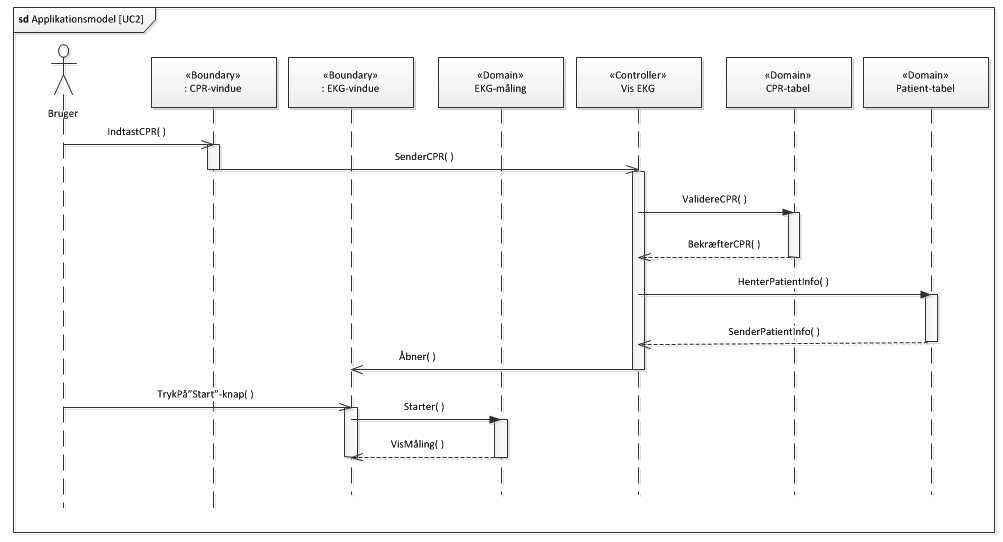
\includegraphics[width=1\textwidth]{Figurer/Snip20150429_33}
	\caption{Sekvensdiagram for UC2}
\end{figure}

\begin{figure}[H]
	\centering
	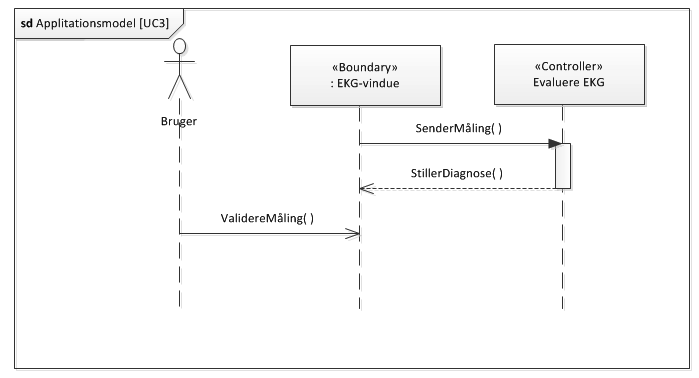
\includegraphics[width=1\textwidth]{Figurer/Snip20150429_31}
	\caption{Sekvensdiagram for UC3}
\end{figure}

\begin{figure}[H]
	\centering
	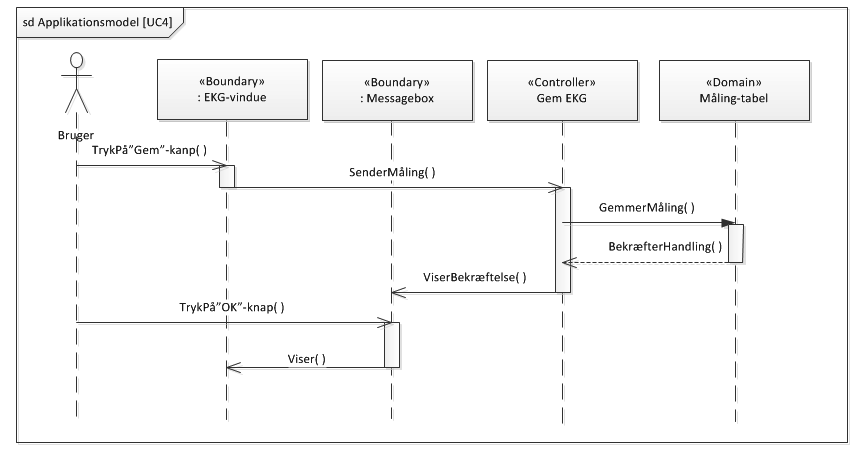
\includegraphics[width=1\textwidth]{Figurer/Snip20150429_28}
	\caption{Sekvensdiagram for UC4}
\end{figure}

\begin{figure}[H]
	\centering
	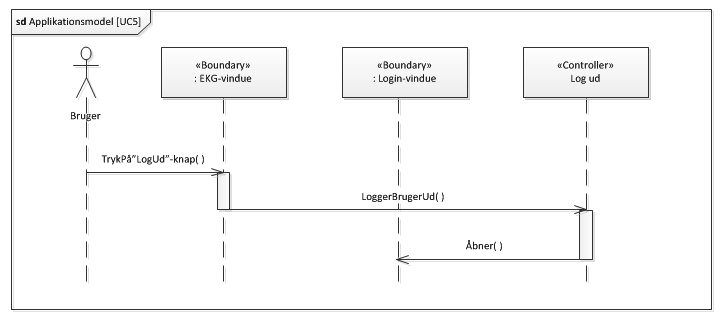
\includegraphics[width=1\textwidth]{Figurer/Snip20150429_30}
	\caption{Sekvensdiagram for UC5}
\end{figure}

\subsubsection{Opdateret Klassediagram}
De opdateret klassediagrammer indeholder metoderne fra de dertilhørende  sekvensdiagrammer - dette giver et overblik over, hvilke metoder de forskellige klasser består af.

\begin{figure}[H]
	\centering
	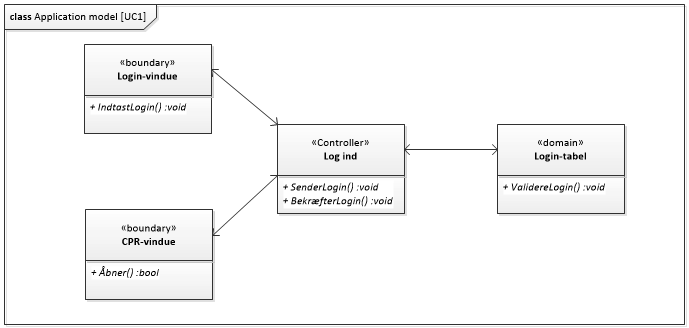
\includegraphics[width=1\textwidth]{Figurer/Snip20150429_20}
	\caption{Klassediagram for UC1}
\end{figure}  

\begin{figure}[H]
	\centering
	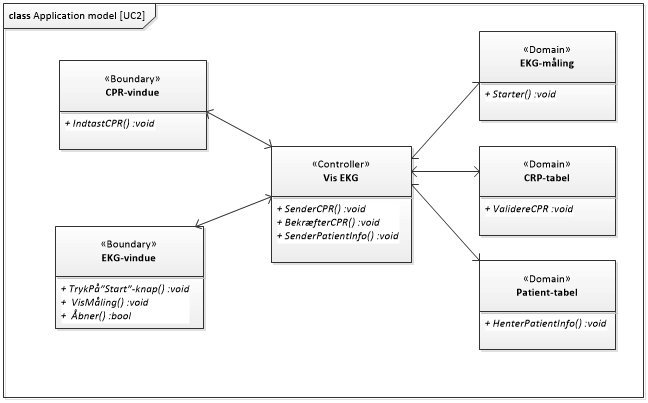
\includegraphics[width=1\textwidth]{Figurer/Snip20150429_22}
	\caption{Klassediagram for UC2}
\end{figure}

\begin{figure}[H]
	\centering
	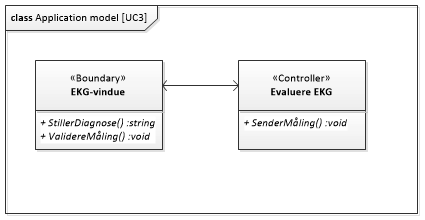
\includegraphics[width=1\textwidth]{Figurer/Snip20150429_23}
	\caption{Klassediagram for UC3}
\end{figure}

\begin{figure}[H]
	\centering
	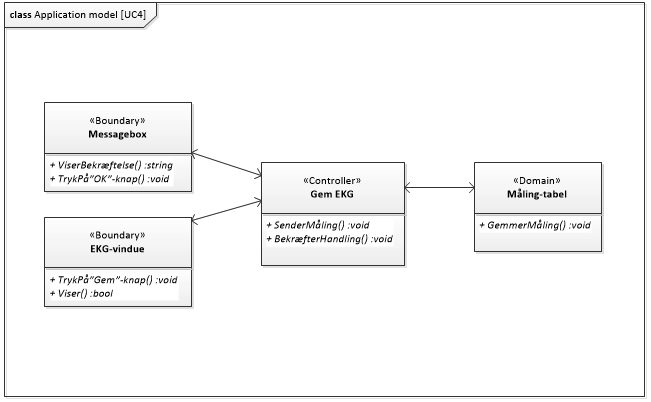
\includegraphics[width=1\textwidth]{Figurer/Snip20150429_26}
	\caption{Klassediagram for UC4}
\end{figure}

\begin{figure}[H]
	\centering
	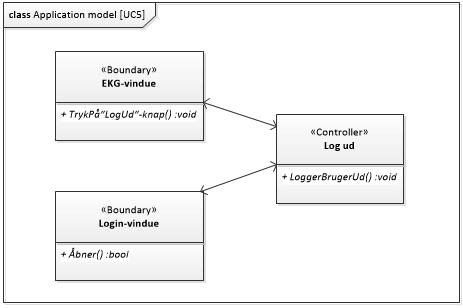
\includegraphics[width=1\textwidth]{Figurer/Snip20150429_25}
	\caption{Klassediagram for UC5}
\end{figure}





